\begin{scanpage}{0138}{120}
\begin{minipage}[t]{.28\linewidth}\vspace{0pt}
\centering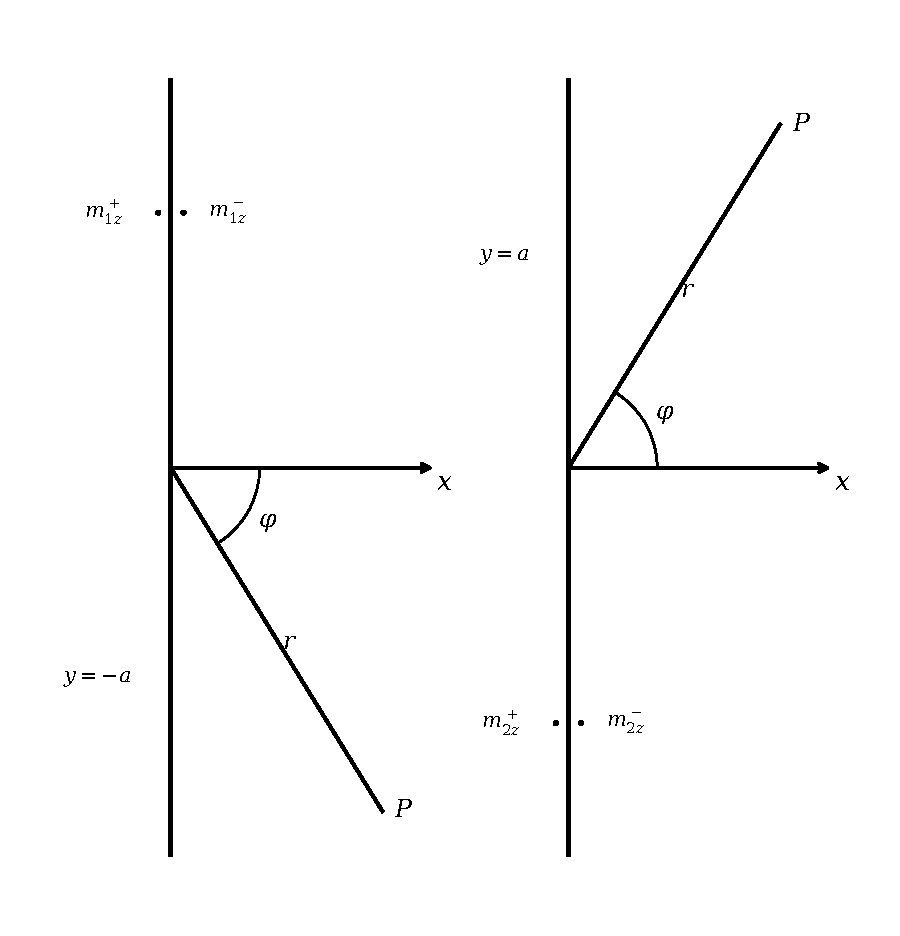
\includegraphics[width=\linewidth]{images/recreated/c-0138-fig.pdf}
\end{minipage}\hfill
\begin{minipage}[t]{.68\linewidth}\vspace{0pt}
\raggedright Figure 47. The problem of secondary diffraction by a strip.\par
$m_{1z}^{+}$ and $m_{1z}^{-}$ are the sources, the fields of which are used when approximating the primary edge wave being propagated from edge 1 ($y=a$);\par
$m_{2z}^{+}$ and $m_{2z}^{-}$ are the sources, the fields from which are used when approximating the primary wave from edge 2 ($y=-a$).
\end{minipage}\par
\[
\begin{aligned}
H_z^-(1)={}&\frac1\pi H_{0z}\widetilde g(1)\!\times\!\int_\infty^{2\sqrt{ka}\cos(\pi/4-\varphi/2)}e^{iq^2}\,dq\,\frac{e^{ikr}}{\sqrt{2kr}}e^{ika(\sin\alpha-\sin\varphi)}\\
&+H_{0z}\widetilde g(1)\frac{e^{i(kr+\pi/4)}}{\sqrt{2\pi kr}}e^{ika(\sin\alpha-\sin\varphi)}
\end{aligned}\tag{21.07}
\]
describes the wave radiated by the source $m_{1z}^{-}$. The sum of these waves equals
\[
\begin{aligned}
H_z(1)={}&\frac2\pi H_{0z}\widetilde g(1)\!\times\!\int_\infty^{2\sqrt{ka}\cos(\pi/4-\varphi/2)}e^{iq^2}\,dq\,\frac{e^{ikr}}{\sqrt{2kr}}e^{ika(\sin\alpha-\sin\varphi)}\\
&+H_{0z}\widetilde g(1)\frac{e^{i(kr+\pi/4)}}{\sqrt{2\pi kr}}e^{ika(\sin\alpha-\sin\varphi)}
\end{aligned}\tag{21.08}
\]
\par The first term in this expression is the desired secondary wave from edge 2, and the second term is the field radiated by the filament which is located above the ideally conducting plane $x=0$ and has the moment
\[
m_{1z}^-=\frac{1}{4\pi k^2}H_{0z}\widetilde g(1)e^{ika\sin\alpha}.\tag{21.09}
\]
where
\[
\widetilde g(1)=g(1)\big|_{\varphi=-\pi/2+0}.\tag{21.10}
\]
\end{scanpage}
